\chapter{机器学习概述与数据特征工程}
\section{引言}
从本章起,本研究将使用机器学习的一般方法对PE患者及正常妊娠孕妇的脉搏波数据进行相关分析研究。
作为过渡章节,本章首先进行了机器学习的一般概述,介绍了机器学习的一般步骤与流程,并明确本研究的机器学习任务。特别地,
在机器学习开始之前,一般还需对使用的数据进行额外的处理工作,即数据特征工程,本章也对这部分的工作内容进行了相应的介绍。

\subsection{本研究的机器学习任务}
\autoref{fig:spml}展示了一个完整的监督学习工程的处理逻辑,主要包含以下步骤\cite{Aurélien2018}:

一、提出具体问题

针对具体情景,明确需要解决的问题及研究目标。

二、数据特征工程

数据特征工程主要包含数据获取、研究数据特性及处理缺失值、标准化等在内的数据准备等内容。

三、训练模型

基于数据探索多种机器学习模型,列出解决问题的最佳模型,对这些模型的超参数进行调整,优化最佳模型。

四、结论与演示

系统地概括总结问题,展示最终解决方案,展示(并解释)以上过程中所出现的现象及问题。

五、生产与部署

准备好最终解决方案的生产环境并进行部署,对系统性能进行监测并定期重新建模等。
\begin{figure}[htbp]
  \centering
  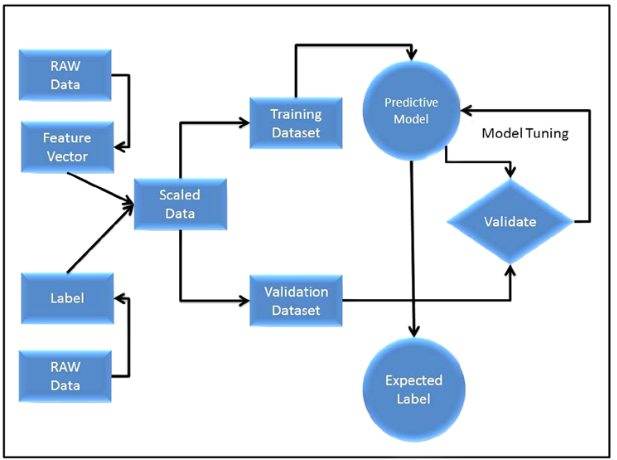
\includegraphics[width=.6\linewidth]{features/spml}
  \caption[监督学习的处理逻辑]{\label{fig:spml}监督学习的处理逻辑\cite{awad2015}}
\end{figure}

回归到本研究的工作内容上来,不难发现,\textbf{探求子痫前期与孕妇脉搏波波形之间的潜在关系}是本研究要具体探索解决的关键性问题。
本文后续内容即为综合应用\textbf{监督学习}与\textbf{无监督学习}的相关算法按上述步骤解决该问题的过程。其中,所有处理程序均在Python环境(Python 3.9.7, 64 bit)下开发完成,
综合使用了Pingouin、Scikit-learn、DESLib及TensorFlow等开源组件工具\cite{python,Vallat2018,scikit-learn,JMLR:v21:18-144,tensorflow2015-whitepaper}。

\section{数据特征工程}
数据特征工程是对原始数据进行一系列工程处理并将其提炼为特征作为输入供算法和模型使用的过程\cite{Zhou2016,Aurélien2018}。
特征工程的核心是表示与展现数据,其本质是去除原始数据中的杂质和冗余,设计更高效的特征以刻画求解的问题与预测模型之间的关系。
下面将对本研究涉及的特征处理进行说明与介绍。

\subsection{数据集的构建}
本文在第三章已经对脉搏波的描述特征参数进行了介绍,这里选取了其中的部分参数构成了基本机器学习的输入数据集。实际上,本研究共构建了三类相互独立的脉搏波描述特征集分别用作特定模型的训练输入数据。

一、波形描述特征集合



二、波形间差异描述特征集合

三、原始波形采样值


本小节对本研究实际采用的多种PPG时域描述特征进行汇总,对各参数符号及前置计算条件也进行了统一说明,如\autoref{tab:allfeatures}所示。
\begin{center}
    \fontsize{10}{4}
    \begin{longtable}{p{3cm}<{\centering}p{1cm}<{\centering}p{2cm}<{\centering}p{6cm}<{\centering}p{1cm}<{\centering}}
        \caption{本研究使用的所有PPG时域指标一览}\\
        \label{tab:allfeatures}\\
        \hline\hline
            \textbf{研究者}&\textbf{时间}&\textbf{脉搏波参数}&\textbf{研究结果}&\textbf{备注}\\
        \hline
        \endfirsthead
        \caption[]{(续)}\\
        \hline
            \textbf{研究者}&\textbf{时间}&\textbf{脉搏波参数}&\textbf{研究结果}&\textbf{备注}\\
        \hline
        \endhead 
        \hline
        \endfoot
        \hline\hline
        \endlastfoot
        &       &       &       &  \\
        &       &       &       &  \\
        &       &       &       &  \\
        &       &       &       &  \\
        &       &       &       &  \\
    \end{longtable}
\end{center}
\subsection{数据集的划分}
在大多数机器学习的案例里,将原始数据集重新划分为训练集与测试集是必不可少的一个步骤。

* 分析数据集准备:两种方式

  * A. by pulse

  * B. by person

\subsection{数据清洗}
* 处理缺失值

\subsection{新特征的创建}
* 构建新特征(char参数)
\subsection{特征相关性验证}
* 分布特性

  * 有无差异性,SPSS统计,已用python实现

  * 特征相关性,heatmap
\subsection{特征缩放}
在大多数情况下,原始数据的特征在数值属性出现较大的比例差异会导致机器学习模型的性能下降、表现欠佳\cite{Aurélien2018}。因此,需要对特征数值的分布进行一定的调整使其称为能够满足具体模型算法的输入要求。
一般的处理原则是同比例缩放所有属性,常见的方法有归一化与标准化两类。

一、归一化

归一化亦称为最小-最大缩放,

二、标准化

balaba
\subsection{特征降维}
事实证明,机器学习模型的训练速度随着训练数据的特征数量增加而降低,这也就是通常而言的维数诅咒或维数灾难。因此,一种可行的策略在构建模型时尽可能只使用“最重要的”特征,即按照特征的贡献度对
原始数据集进行降维处理。但需要注意的是,数据降维在加速训练的同时,通常也会导致系统性能的下降。从这个角度说,特征降维是机器学习过程中的一个可选项而非必选项。

由于特征降维在划分上是数据特征工程的一部分,但在逻辑上的处理又往往与具体的机器学习模型绑定。故本小节暂时只进行概念,真正的降维分析请参见本文后续章节内容。
\section{小结}